\documentclass{article}
\usepackage[utf8]{inputenc}
\usepackage[margin=0.70in]{geometry}
\usepackage{hyperref}
\usepackage{graphicx}
\usepackage{authblk}
\usepackage{subfig}
\usepackage{indentfirst}
\usepackage{minted}

\title{Program Assignment 3B: Quantum Simulation Optimizations}
\author{Brian Park}
\affil{North Carolina State University, Computer Engineering 786}
\date{April 2023}

\begin{document}

\maketitle

\section{Naive Multi-Gated Quantum Simulation}
To write quantum simulation on six single qubit quantum gates to six different qubits on an $n$-qubit quantum circuit, I used the same implementation from Project 1A, but repeated the process six times. As a result, I had to add intermediate kernels to copy device-to-device memory of output back into the input (the \verb|cudaMemcpy| was too slow). Also, I had to add synchronizations via \verb|__syncthreads()|. Although there are implicit barriers between kernel functions in CUDA, it was necessary to add synchronization barriers within the kernel. This was because when a kernel is launched, there is no guarantee that a warp will finish its execution as it's not required to wait until the first warp exits. Thus, a kernel-level synchronization primitive was added. 

\begin{minted}{Cuda}[H]
__global__ void quantum_simulation_gpu(const float* U, const float* a, float* output, int qubit,
                                       int N) {
    int tid = blockDim.x * blockIdx.x + threadIdx.x;

    register size_t qid = 1 << qubit;

    if (tid > N)
        return;

    if (tid & qid)
        output[tid] = U[2] * a[tid - qid] + U[3] * a[tid];
    else
        output[tid] = U[0] * a[tid] + U[1] * a[tid + qid];
    __syncthreads();
}
\end{minted}

Furthermore, the main execution of kernels look like this:

\begin{minted}{C}[H]
quantum_simulation_gpu<<<blocksPerGrid, threadsPerBlock>>>(U_0_gpu, a_gpu, output_gpu, qubit_0,
                                                            a.size());
device_to_device_memcpy<<<blocksPerGrid, threadsPerBlock>>>(output_gpu, a_gpu, a.size());
quantum_simulation_gpu<<<blocksPerGrid, threadsPerBlock>>>(U_1_gpu, a_gpu, output_gpu, qubit_1,
                                                            a.size());
device_to_device_memcpy<<<blocksPerGrid, threadsPerBlock>>>(output_gpu, a_gpu, a.size());
quantum_simulation_gpu<<<blocksPerGrid, threadsPerBlock>>>(U_2_gpu, a_gpu, output_gpu, qubit_2,
                                                            a.size());
device_to_device_memcpy<<<blocksPerGrid, threadsPerBlock>>>(output_gpu, a_gpu, a.size());
quantum_simulation_gpu<<<blocksPerGrid, threadsPerBlock>>>(U_3_gpu, a_gpu, output_gpu, qubit_3,
                                                            a.size());
device_to_device_memcpy<<<blocksPerGrid, threadsPerBlock>>>(output_gpu, a_gpu, a.size());
quantum_simulation_gpu<<<blocksPerGrid, threadsPerBlock>>>(U_4_gpu, a_gpu, output_gpu, qubit_4,
                                                            a.size());
device_to_device_memcpy<<<blocksPerGrid, threadsPerBlock>>>(output_gpu, a_gpu, a.size());
quantum_simulation_gpu<<<blocksPerGrid, threadsPerBlock>>>(U_5_gpu, a_gpu, output_gpu, qubit_5,
                                                            a.size());
\end{minted}

Because I wrote multiple kernels, it also meant more accesses to global memory. As a result, there are 11 kernels, and 11 global reads and writes reported in GPGPU-Sim. The number of global reads is 576320 and global writes is 32768. In total, there are 609088 global memory accesses. 

\section{Multi-Gated Quantum Simulation with Shared Memory Optimization}
The next step was to apply optimizations to make the code run efficiently. To do this, I used the SharedMem method as mentioned in HyQuas \cite{hyquas}. This required to split the input vector in to fragments of size 64 elements. I chose 64 specifically to fit in the $2^6$ elements for the six qubit offsets. Before the kernel is called, there are some bit manipulations that needed to be done to reshuffle the indices for the input vector into an auxillary array. I followed the figure from HyQuas shown in Figure 1 to do that manipulation from global index to shared index. Then I applied the gates sequentially per fragment. Then remap and restore the indices from shared index back to global index to store back to global memory. In order to map the gates correctly, as the first gate will couple with even and odd indices, second gate will couple with elements 2 indices apart, third gate will couple with elements 4 indices apart, etc, I had to do additional bit manipulations to compute the offset within shared memory buffer. 

\begin{figure}[H]
    \centerline{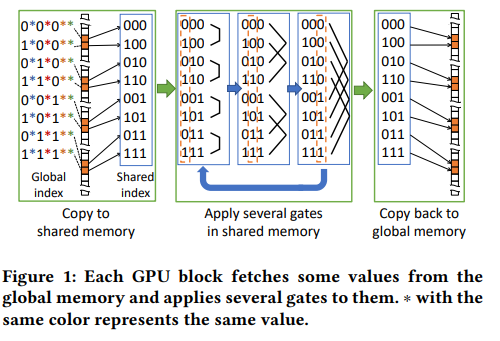
\includegraphics[width=6in]{sharedmem.png}}
\end{figure}

Below, is what the GPU kernel looks like for the shared memory optimization. 

\begin{minted}{Cuda}[H]
__global__ void quantum_simulation_gpu(float* U_0, float* U_1, float* U_2, float* U_3, float* U_4,
                                       float* U_5, float* a, float* output, size_t N,
                                       size_t* auxillary_array, size_t* offsets) {
                                       
    int tid = blockDim.x * blockIdx.x + threadIdx.x;

    if (tid >= N / 2) {
        return;
    }

    __shared__ float a_shared[FRAGMENT_SIZE];

    // Load the fragment from global memory to shared memory
    size_t offset = offsets[blockIdx.x];

    size_t idx = threadIdx.x * 2;

    a_shared[idx] = a[auxillary_array[idx] + offset];
    a_shared[idx + 1] = a[auxillary_array[idx + 1] + offset];

    float* Us[6] = {U_0, U_1, U_2, U_3, U_4, U_5};
    __syncthreads();
    __syncwarp();

    register float x0, x1;
    for (size_t gate = 0; gate < 6; gate++) {
        float* U = Us[gate];
        size_t gate_offset = 1 << gate;

        if ((idx & gate_offset) == 0) {
            x0 = a_shared[idx];
            x1 = a_shared[idx + gate_offset];

            a_shared[idx] = U[0] * x0 + U[1] * x1;
            a_shared[idx + gate_offset] = U[2] * x0 + U[3] * x1;
        } else {
            x0 = a_shared[idx - gate_offset + 1];
            x1 = a_shared[idx + 1];

            a_shared[idx - gate_offset + 1] = U[0] * x0 + U[1] * x1;
            a_shared[idx + 1] = U[2] * x0 + U[3] * x1;
        }
        __syncthreads();
        __syncwarp();
    }

    // Store the fragment from shared memory to global memory
    output[auxillary_array[idx] + offset] = a_shared[idx];
    output[auxillary_array[idx + 1] + offset] = a_shared[idx + 1];
    return;
\end{minted}

In the end, only one kernel is called as a result:

\begin{minted}{C}[H]
quantum_simulation_gpu<<<blocksPerGrid, threadsPerBlock>>>(
    U_0_gpu, U_1_gpu, U_2_gpu, U_3_gpu, U_4_gpu, U_5_gpu, a_gpu, output_gpu, a.size(),
    auxillary_array_gpu, offsets_gpu);
\end{minted}


There are 19168 global reads and 32768 global writes. Thus, amounting to a total of 51936 global memory accesses. There are far less global memory accesses ($30\times$) than the naive version.

% 3. Use GPGPU-SIM to count the number of global memory accesses of task1 and task2, report the count number of task1 and task2 and analyze their differences in your report.

\section{Multi-Gated Quantum Simulation with Thread Coarsening Optimization}
I have already applied a bit of thread coarsening or thread fusion, but using 32 threads per 64 elements. I can improve this further by performing 16 threads over 64 elements, such that 1 thread operates over 4 elements. In order to do that, I unrolled the loop twice. Unfortunately, that creates the same number of reads (19168), but twice the number of global writes (65536). This is mainly because I have to write to more temporary variables. Unfortunately, I see no efficient way to optimize even more, due to the coupling of gates and indices of shared memory. If I were to merge if-else statements, I would run into even more performance decrease, as there are less threads running in parallel. I also tried to unroll the loops at the gate level, but found no benefit as it incurs more overhead due to synchronization that is required in the inner for loop to update the output values. 


\begin{minted}{Cuda}[H]
__global__ void quantum_simulation_gpu(float* U_0, float* U_1, float* U_2, float* U_3, float* U_4,
                                       float* U_5, float* a, float* output, size_t N,
                                       size_t* auxillary_array, size_t* offsets) {

    int tid = blockDim.x * blockIdx.x + threadIdx.x;

    if (tid >= N / 4) {
        return;
    }

    __shared__ float a_shared[FRAGMENT_SIZE];

    // Load the fragment from global memory to shared memory
    size_t offset = offsets[blockIdx.x];

    size_t idx = threadIdx.x * 4;

    a_shared[idx] = a[auxillary_array[idx] + offset];
    a_shared[idx + 1] = a[auxillary_array[idx + 1] + offset];
    a_shared[idx + 2] = a[auxillary_array[idx + 2] + offset];
    a_shared[idx + 3] = a[auxillary_array[idx + 3] + offset];

    float* Us[6] = {U_0, U_1, U_2, U_3, U_4, U_5};
    __syncthreads();
    __syncwarp();

    register float x0, x1;
    for (size_t gate = 0; gate < 6; gate++) {
        float* U = Us[gate];
        size_t gate_offset = 1 << gate;
        if ((idx & gate_offset) == 0) {
            x0 = a_shared[idx];
            x1 = a_shared[idx + gate_offset];

            a_shared[idx] = U[0] * x0 + U[1] * x1;
            a_shared[idx + gate_offset] = U[2] * x0 + U[3] * x1;
        } else {
            x0 = a_shared[idx - gate_offset + 1];
            x1 = a_shared[idx + 1];

            a_shared[idx - gate_offset + 1] = U[0] * x0 + U[1] * x1;
            a_shared[idx + 1] = U[2] * x0 + U[3] * x1;
        }

        if (((idx + 2) & gate_offset) == 0) {
            x0 = a_shared[idx + 2];
            x1 = a_shared[idx + 2 + gate_offset];

            a_shared[idx + 2] = U[0] * x0 + U[1] * x1;
            a_shared[idx + 2 + gate_offset] = U[2] * x0 + U[3] * x1;
        } else {
            x0 = a_shared[idx - gate_offset + 3];
            x1 = a_shared[idx + 3];

            a_shared[idx - gate_offset + 3] = U[0] * x0 + U[1] * x1;
            a_shared[idx + 3] = U[2] * x0 + U[3] * x1;
        }
        __syncthreads();
        __syncwarp();
    }

    // Store the fragment from shared memory to global memory
    output[auxillary_array[idx] + offset] = a_shared[idx];
    output[auxillary_array[idx + 1] + offset] = a_shared[idx + 1];
    output[auxillary_array[idx + 2] + offset] = a_shared[idx + 2];
    output[auxillary_array[idx + 3] + offset] = a_shared[idx + 3];
    return;
}
\end{minted}

\section{Conclusion}
Here, I compare all of the implementations to understand the impact of each optimization. I benchmarked this on \verb|input_for_qc16_q0_q2_q4_q6_q8_q10.txt| as that is the largest dataset. The results shown previously and below are on V100 config. Real hardware benchmarks were done on RTX 2080. Correctness was verfied on Hydra clusters as well. But Thread Coarsening gives no benefit due to how the algorithm and data movement works. 

\begin{figure}[H]
    \centerline{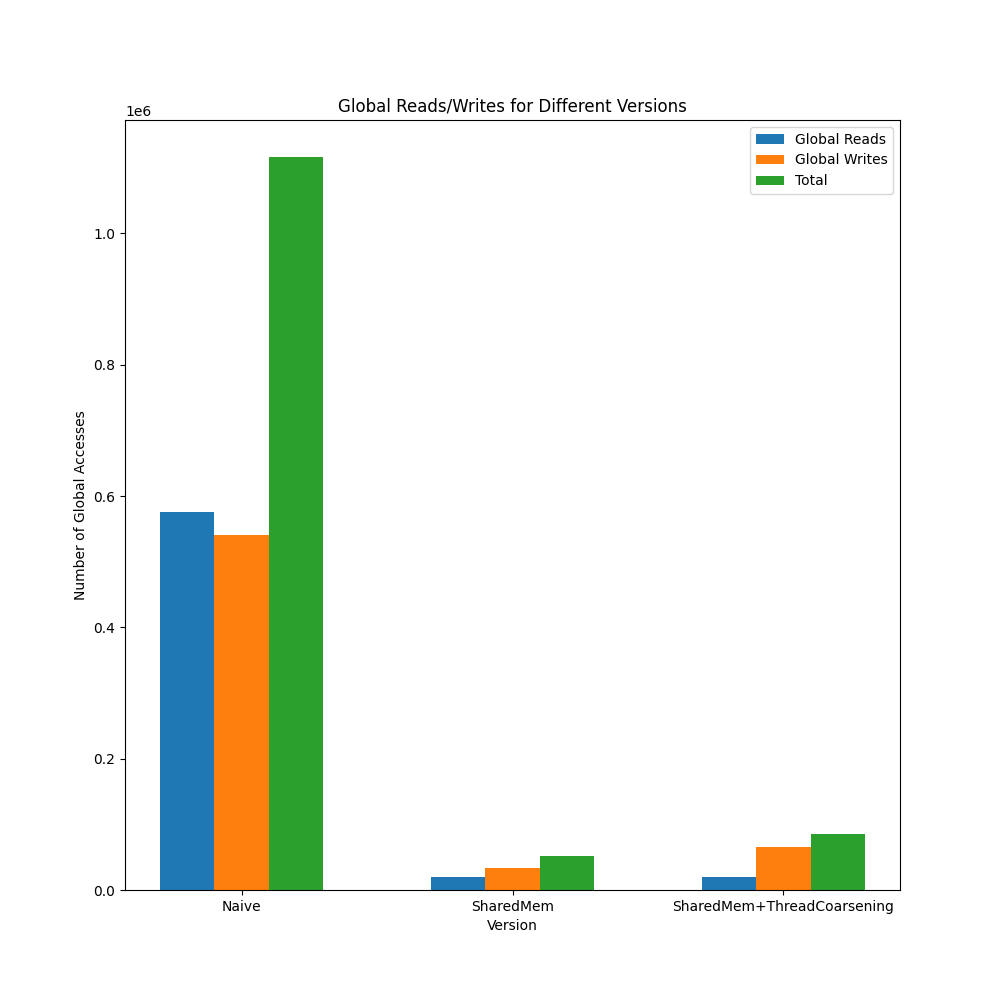
\includegraphics[width=6in]{global_reads_writes.png}}
\end{figure}

\begin{figure}[H]
    \centerline{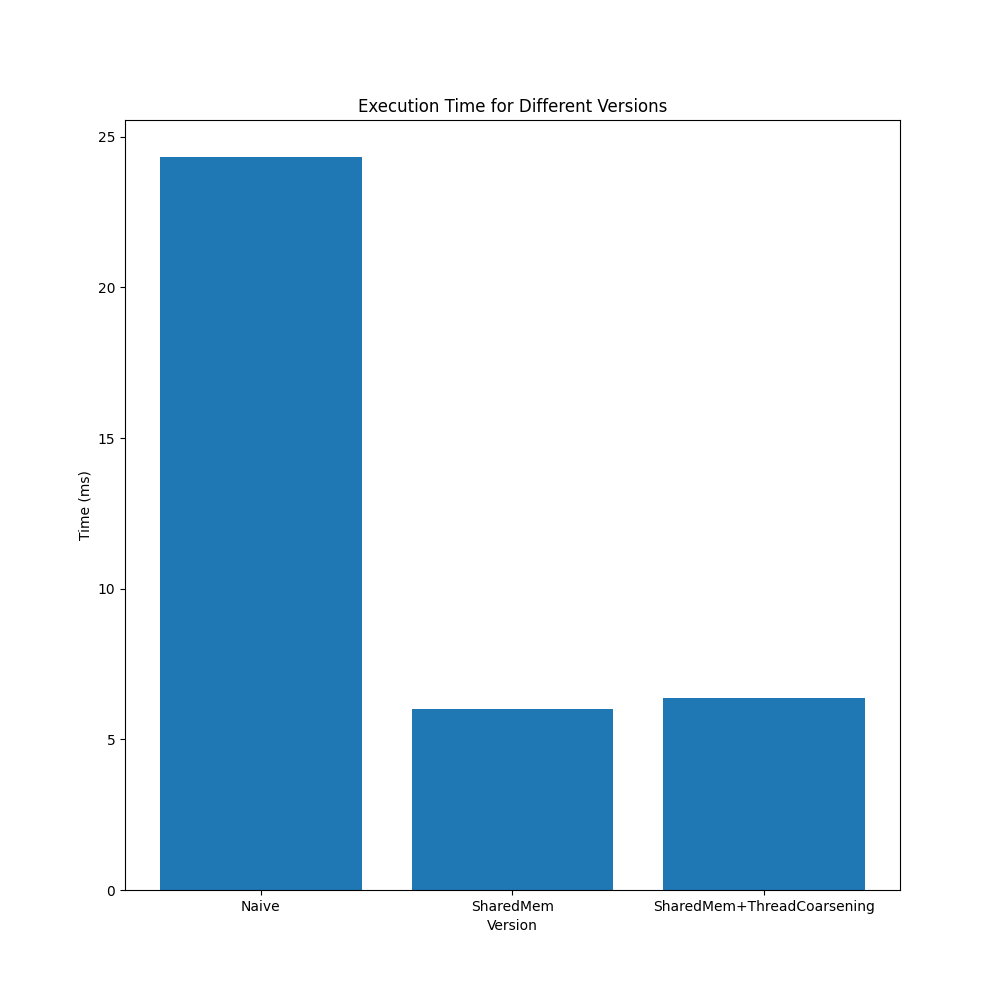
\includegraphics[width=6in]{quantum_time.png}}
\end{figure}

We see that SharedMem performs the best, with Thread Coarsening coming very close. Sometimes, if code is not highly parallelizable with deep reuse, like matrix multiplication, thread coarsening may have diminishing returns. And we see that is the case here with quantum simulation. In the end, SharedMem method gives us $4\times$ performance gains against the naive implementation. 

\bibliographystyle{ieeetr}
\bibliography{references}

\end{document}
